The given curve,
% \begin{align}
% y&=\frac{{x-1}}{{x-2}} 
% \end{align}
 can be expressed as,
\begin{align}
yx-2y-x+1 =0
\label{quadform/75/2.0.1}
\end{align}
yielding
\begin{align}
\vec{V}&=\myvec{\frac{1}{2} & 0 \\ 0 & \frac{1}{2}},\vec{V}^{-1}=\myvec{0&2\\2&0}\vec{u}=\myvec{-\frac{1}{2}\\-1},
f =1 \label{quadform/75/2.0.3}
\end{align}
\begin{align}
\because  |\vec{V}| < 0
\end{align}
 \eqref{quadform/75/2.0.1} is a hyperbola.
Let the slope of tangent be $r$. Then the  direction vector and normal vector of tangent to \eqref{quadform/75/2.0.1} are
\begin{align}
    \vec{m}&= \myvec{1\\r},\vec{n}=\myvec{r\\-1} \label{quadform/75/2.0.5}\\
\kappa=&\pm \sqrt{\frac{\vec{u^T}\vec{V}^{-1}\vec{u}-\vec{f}}{\vec{n^T}\vec{V}^{-1}\vec{n}}}\\
&=\sqrt{\frac{-1}{4r}} \label{quadform/75/2.0.8}
\end{align}
For hyperbola, the point of contact for the tangent is
\begin{align}
\vec{q}&=\vec{V}^{-1}(\kappa\vec{n}-\vec{u})\label{quadform/75/2.0.6}\\
\implies \vec{V}\vec{q}+\vec{u}&=\kappa\vec{n}\\
\implies \myvec{\frac{1}{16}\\4}&=\kappa\vec{n} \quad ( \text{ From } \quad \eqref{quadform/75/2.0.3})\\
\implies \myvec{\frac{1}{16}\\4}&=\sqrt{\frac{-1}{4r}}\myvec{r\\-1}\\
\implies \myvec{\frac{1}{16}\\4}&=\myvec{r\sqrt{\frac{-1}{4r}}\\-\sqrt{\frac{-1}{4r}}}\\
\implies -\sqrt{\frac{-1}{4r}}&=4\\
\implies r &= -\frac{1}{64}
\end{align}
which is the desired slope. Fig.     \ref{quadform/75/fig:Tangent to HYPERBOLA.} verifies this result.
\begin{figure}[!ht]
    \centering
    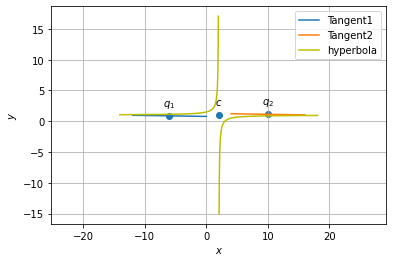
\includegraphics[width=\columnwidth]{solutions/su2021/2/75/HYPERBOLA.png}
    \caption{Tangent to HYPERBOLA.}
    \label{quadform/75/fig:Tangent to HYPERBOLA.}
\end{figure}  


